\chapter{Reproducing symmetry-based disentangled representation learning}

\whendraft{
\noindent\rule{\textwidth}{1mm}
\textbf{Section to do:}
\begin{enumerate}
    \item 
\end{enumerate}
\noindent\rule{\textwidth}{1mm}
}


Our objective for this chapter is to validate our framework by showing it can reproduce Symmetry-based disentangled representation learning (SBDRL), a well-establish mathematical framework for disentanglement in representation learning.

%%%%%%%%%%%%%%%%%%%%%%%%%%%%%%%%
\section{Motivation}

SBDRL is a well-established mathematical framework for disentanglement in representation learning based on group actions.

\draftnote{blue}{awjdean}{Put more on the significance of SBDRL.}

We will now reproduce SBDRL using our framework; we do this for the following reasons:
\begin{enumerate}[(1)]
    \item Showing that our framework can accommodate a known, structured representation paradigm provides a good validation step for our framework;
    \item Reproducing SBDRL using a more fundamental framework could allow us to identify limitations with the SBDRL framework;
    \item Reproducing SBDRL using a more fundamental framework could allow us to generalise the key concepts of SBDRL to more complicated scenarios.
\end{enumerate}

%%%%%%%%%%%%%%%%%%%%%%%%%%%%%%%%
\section{Description of SBDRL}

The SBDRL framework treats agents as experiencing the world through a map $f = h \circ b: W \to Z$ made from the composition of a generative process $b: W \to O$ and a $h: O \to Z$, where $W$ is a set of world states, $O$ is a set of observation states, and $Z$ is a set of agent representation states.
The framework treats the map $f$ as bijective\footnote{\draftnote{blue}{awjdean}{Footnote: Mention how they explain away cases where $f$ is not injective and $f$ is not surjective.}.}.

\paragraph{Symmetry-based representations.}
SBDRL assumes that the set $W$ of world states has a set $G$ of symmetries that form a group.
This group $G$ acts on the set $W$ of world states via a group action $\cdot_{W}: G \times W \to W$.
For the agent's representation states $z \in Z$ to be symmetry-based representations, the corresponding group action $\cdot_{Z}: G \times Z \to Z$ of $G$ on $Z$ must exist.

SBDRL involves the agent learning in a way that aligns the agent's representations so that they respect the group action $\cdot_{Z}$, which means the symmetries in the representations reflect the symmetries of the world states.

The mathematical condition for SBDRs is:
\begin{equation}\label{eqn: SBRs eqn}
    f(g \cdot_{W} w) = g \cdot_{Z} f(w) \quad \text{for all $w\in W$, for all $g \in G$}
\end{equation}
In words, applying any action $g \cdot_{W}$ of a symmetry element $g \in G$ to any world state $w \in W$ and then applying the mapping $f$ gives the same result as first applying the mapping $f$ to $w$ to give a representation state $f(w) \in Z$ and then applying the action $g \cdot_Z$ of the same symmetry element $g \in G$ to the representation state $f(w) \in Z$.
When equation \ref{eqn: SBRs eqn} is satisfied, then $f$ is called a \emph{group-equivariant map}.

\paragraph{Symmetry-based disentangled representations.}
The SBDRL framework now assumes the group $G$ of symmetries of the world states in $W$ decomposes as a direct product $G = G_1 \times \hdots \times G_i \times \hdots \times G_n$.
They say that the group action $\cdot_Z : G \times Z \to Z$ and the set $Z$ are \emph{disentangled with respect to the decomposition of $G$}, if there is a decomposition $Z = Z_1 \times \hdots \times Z_i \times \hdots \times Z_n$ and actions $\cdot_{Z_i}: G_i \times Z_i \to Z_i, i \in \{1, \hdots, n\}$ such that $(g_{G_1}, g_{G_2},...) \cdot_Z (z_{Z_1}, z_{Z_2},...) = (g_{G_1} \cdot_{Z_1} z_{Z_1}, g_{G_2} \cdot_{Z_2} z_{Z_2},...)$, where $g_{G_i} \in G_i$ and $z_{Z_i} \in Z_i$.
In other words, each subspace $Z_i$ is invariant to the action of all the $G_{j \neq i}$ and only affected by $G_i$.

\paragraph{Summary.}
There is a bijective map $f: W \to Z$.
The representation states in $Z$ are symmetry-based disentangled with respect to the decomposition $G = G_1 \times \hdots \times G_i \times \hdots \times G_n$ if:
\begin{enumerate}[(1)]
    \item There exists a group action $\cdot_{W}: G \times W \to W$ and a corresponding group action $\cdot_{Z}: G \times Z \to Z$;
    \item The map $f : W \to Z$ is group-equivariant between the group actions on $W$ and $Z$: $g \cdot_{Z} f(w) = f(g \cdot_{W} w)$.
    
    In other words, the diagram
    % https://q.uiver.app/#q=WzAsNCxbMCwwLCJ3Il0sWzIsMCwiZyBcXGNkb3Rfe1d9IHciXSxbMCwyLCJmKHcpIl0sWzIsMiwiZyBcXGNkb3Rfe1p9IGYodykgPSBmKGcgXFxjZG90X3tXfSB3KSJdLFswLDEsImcgXFxjZG90X3tXfSJdLFswLDIsImYiLDJdLFsxLDMsImYiLDJdLFsyLDMsImcgXFxjZG90X3tafSJdXQ==
\[\begin{tikzcd}
	w && {g \cdot_{W} w} \\
	\\
	{f(w)} && {g \cdot_{Z} f(w) = f(g \cdot_{W} w)}
	\arrow["{g \cdot_{W}}", from=1-1, to=1-3]
	\arrow["f"', from=1-1, to=3-1]
	\arrow["f"', from=1-3, to=3-3]
	\arrow["{g \cdot_{Z}}", from=3-1, to=3-3]
\end{tikzcd}\]

    commutes.    

    \item There exists a decomposition of the representation $Z = Z_1 \times \hdots \times Z_n$ such that each subspace $Z_i$ is only affected by the action $G_i$ and is unaffected by the actions $G_{j \neq i}$.
\end{enumerate}

If $W$, $Z$, and $f$ satisfy conditions (1) and (2), then the agent's representation is a symmetry-based.
If $W$, $Z$, and $f$ satisfy conditions (1), (2), and (3) then the agent's representation is a symmetry-based disentangled.

\whendraft{
\noindent\rule{\textwidth}{1mm}
\textbf{To do:}
\begin{enumerate}
    \item Reproduce figure showing map $f: W \to Z$.
\end{enumerate}
\noindent\rule{\textwidth}{1mm}
}

%%%%%%%%%%%%%%%%%%%%%%%%%%%%%%%%
\section{SBDRL in our framework}

\subsection{Set up}
\draftnote{blue}{awjdean}{Make improvements here!}

The agent in the SBDRL framework is equivalent in our framework to a Markov blanket agent embodied in the world with ideal sensors.
For simplicity we will initially only consider worlds where all the transformations of the world are due to the actions of an agent\footnote{We will discuss worlds where the transformations are not due to the actions of an agent later.}.

In the SBDRL framework, the group actions $G \times W \to W$ acts as functions $\cdot_{W}: W \to W$ that move the world from one world state to another.
In other words, the effect of applying each group element $g \in G$ is made up of a collection of transformations of the world between different world states, and so the action of each group element is a function $g \cdot_{W}: W \to W$; when considering group actions only due to the actions of an agent, these functions $g \cdot_{W}: W \to W$ are the functions $*_{a}: W \to W$ in our framework\footnote{\autocite{caselles2019symmetry} also makes this connection between the symmetry transformations of SBDRL and the actions of an agent; however, they stop at actions that cannot form a group (e.g., irreversible actions), while we will use our framework to explore the algebra of worlds that cannot form a group.}.

The SBDRL formalism implicitly considers transformations that 
start and end in the same world state as the same.
In our framework, this is analogous to applying the equivalence relation $\sim$ to construct the quotient set $\hat{A}^{*}/\sim$.

\begin{table}[H]
    \centering
    \begin{tabular}{|c|c|c|c|}
         & Our framework    & SBDRL     & Caselles-Dupre \\
         \hline
         States of the world & $W$ & $W$ & $W$ \\
         Actions causing dynamics of world & $a* = *_{a}: W \to W$ & $g \cdot_{W}: W \to W$ & $f(\_, a_{t}): W \to W$ \\
         Agent & Embodied agent with ideal sensors & Map $f: W \to Z$ is bijective & Embodied agent, map $W \to Z$ is bijective
    \end{tabular}
    \caption{Caption}
    \label{tab:my_label}
\end{table}

We want to answer the question:
\begin{center}
    In a world where transformations occur solely due to the actions of an embodied agent, what structure must the world possess for the transformations of the world to form a group?
\end{center}


Essentially, we want $(\hat{A}^{*}/\sim) \times W \to W$ to be a (global) group action.


%%%%%%%%%%%%%%%%%%%%%%%%%%%%%%%%
\section{Example: $\mathscr{W}_{(2,2)C}$}

We will now show that the example world $\mathscr{W}_{(2,2)C}$ that we used in section \ref{sec:A mathematical treatment of worlds and their transformations} produces a group action $(\hat{A}^{*}/\sim \times W \to W$ is a group action (i.e., $(\hat{A}^{*}/\sim, \circ_{\sim})$ a group).










\whendraft{
\noindent\rule{\textwidth}{1mm}
\textbf{Up next:}
\begin{enumerate}
    \item \sout{Agent stuff.}
    \item \sout{Higgins --> equivalence relation.}
    \item Mention that SBDRL requires a global group action.
\end{enumerate}

\textbf{To do:}
\begin{enumerate}
    \item Mention: we want to initially consider worlds where the entire action transformation structure forms a group.
    Later we will consider worlds where $\hat{A}^{*}$ contains a (global) group through colimits.
    \item State that $\mathscr{W}_{(2,2)C}$ can give SB representations.
\end{enumerate}
\noindent\rule{\textwidth}{1mm}
}

%%%%%%%%%%%%%%%%%%%%%%%%%%%%%%%%%%%%%%%%%


\whendraft{
\noindent\rule{\textwidth}{1mm}






\noindent\rule{\textwidth}{1mm}
%%%%%%%%%%%%%%%%%%%%%%%%%%%%%%%%%%%%%%%%%%%%%%%
\section{Reproducing SBDRL}\label{sec:Reproducing SBDRL}

We will now use the framework set out in the previous section to reproduce the SBDRs of \cite{Higgins2018}.
We illustrate our ideas using the worlds that are similar to those given by \cite{Higgins2018} and \cite{caselles2019symmetry}.
We choose to begin by reproducing symmetry-based representations using our framework because (1) symmetry-based representations describe transformations of the world that have formed relatively simple and well-understood algebraic structures (groups), (2) groups, and the symmetries they describe, are gaining increasing prominence in artificial intelligence research, (3) it shows how our framework encompasses previous work in formalising the structure of transformations of a world, and (4) it provides a more rigorous description of SBDRL, which should aid future analysis and development of the concept.

Section \textbf{sec:Symmetry-based disentangled representation learning} provides a description of SBDRL, and Section \textbf{sec:SBDRL through equivalence} shows how to get to SBDRL using an equivalence relation on the actions of the agent.
Section \textbf{sec:Algorithmic exploration of world structures} provides information on the algorithmic exploration of world structures performed on example worlds.
Section \textbf{sec:Example} goes through a worked example.
Finally, Section \textbf{sec:World conditions} shows the conditions of the world that are required for the actions of an agent to be fully described by SBDRs.

%%%%%%%%%%%%%%%%%%%%%%%%%%%%%%%%%%%%%%%%%%%%%%%
%%%%%%%%%%%%%%%%%%%%%%%%%%%%%%%%%%%%%%%%%%%%%%%
\subsection{Symmetry-based disentangled representation learning}\label{sec:Symmetry-based disentangled representation learning}

We will now present a more detailed description of the SBDRL formalism.

\paragraph{From world states to representation states}
The world state is an element of a set $W$ of all possible world states.
The observations of a particular world state made by the agent's sensors are elements of the set $O$ of all possible observations.
The agent's internal state representation of the world state is an element of a set $Z$ of all possible internal state representations.
There exists a composite mapping $f = h \circ b: W \to Z$ that maps world states to states of the agent's representation ($w \mapsto z$); this composite mapping is made up of the mapping of an observation process $b: W \to O$ that maps world states to observations ($w \mapsto o$) and the mapping of an inference process $h: O \to Z$ that maps observations to the agent's internal state representation ($o \mapsto z$) (see Figure \ref{fig:observation-maps}).

\begin{figure}[t]
	\centering
	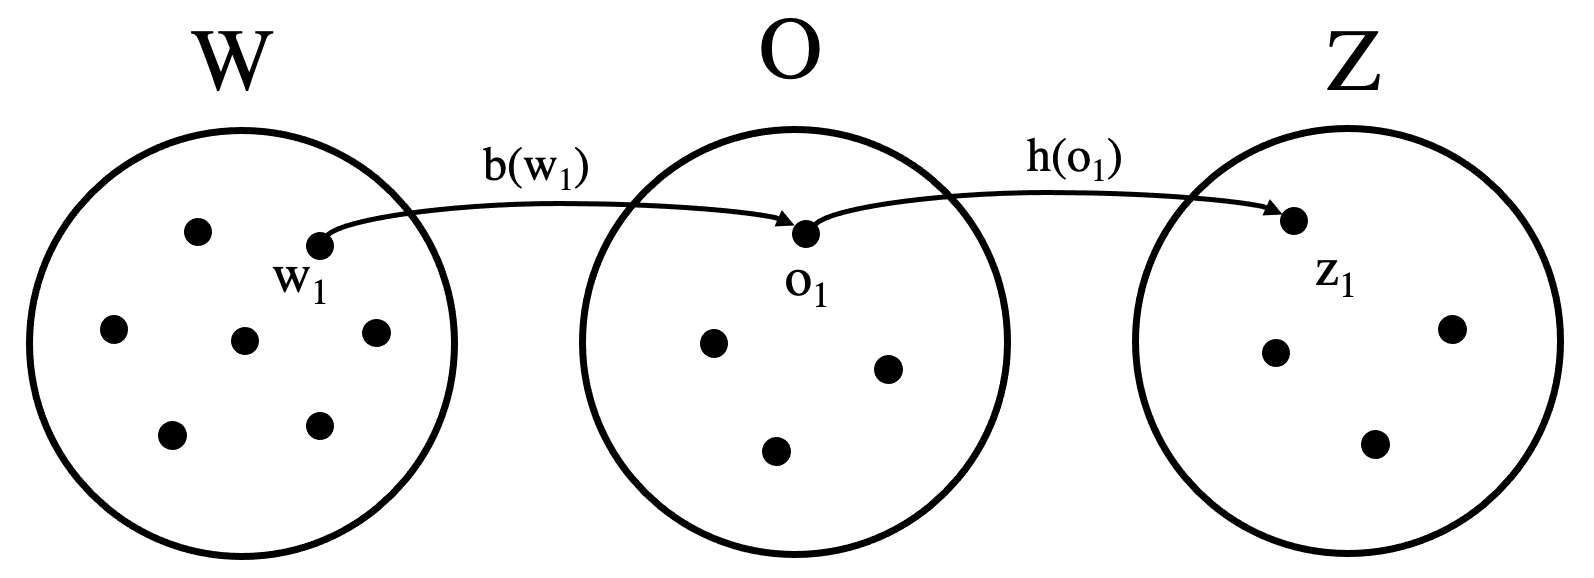
\includegraphics[scale = 0.35]{3ReproducingSBDRL/Old/Images/W_to_O_to_Z_mapping.png}
	\caption{The composite mapping from the set $W$ of world states to the set $Z$ of state representations via the set $O$ of observations.}
	\label{fig:observation-maps}
\end{figure}

\paragraph{Groups and symmetries}
\begin{definition}[Group]
	A group $G$ is a set with a binary operation $G \times G \to G$, $(g, g') \mapsto g \circ g'$ called the \textit{composition} of group elements that satisfies the following properties:
	\begin{enumerate}
		\item \textit{Closure.}
		      $g \circ g'$ is defined for all $g, g' \in G$.
		\item \textit{Associative.}
		      $(g \circ g') \circ g'' = g \circ (g' \circ g'')$ for all $g, g', g'' \in G$.
		\item \textit{Identity.}
		      There exists a unique identity element $1 \in G$ such that $1 \circ g = g \circ 1 = g$ for all $g \in G$.
		\item \textit{Inverse.}
		      For any $g \in G$, there exists $g^{-1} \in G$ such that $g \circ g^{-1} = g^{-1} \circ g = 1$.
	\end{enumerate}
\end{definition}

Applying symmetries to objects is mathematically defined as a \textit{group action}.

\begin{definition}[Group action]
	Given a group $G$ and a set $X$, a group action of $G$ on $X$ is a map $G \times X \to X$, $(g,x) \mapsto g * x$ that satisfies the following properties:
	\begin{enumerate}
		\item \textit{Compatibility with composition.}
		      The composition of group elements and the group action are compatible: $g' \circ (g * x) = (g' \circ g) * x$ for $g,g' \in G$ and $x \in X$.
		\item \textit{Identity.}
		      The group identity $1 \in G$ leaves the elements of $X$ unchanged: $1 * x = x$ for all $x \in X$.
	\end{enumerate}
\end{definition}



Another important property of groups is commutation.
Two elements of a group \textit{commute} if the order they are composed does not matter: $g \circ g' = g' \circ g$.
If all elements in a group commute with each other then the group is called \textit{commutative}.
Subgroups of a group might commute with each other.

\paragraph{\sout{Symmetry-based representations}}
\sout{
	The set $W$ of world states has a set of symmetries that are described by the group $G$.
	This group $G$ acts on the set $W$ of world states via a group action $\cdot_{W}: G \times W \to W$.
	For the agent's representations $z_i \in Z$ to be symmetry-based representations, a corresponding group action $\cdot_{Z}: G \times Z \to Z$ must be found so that the symmetries of the agent's representations reflect the symmetries of the world states.
	The mathematical condition for this is that, for all $w \in W$ and all $g \in G$, applying the action $g \cdot_W$ to $w$ and then applying the mapping $f$ gives the same result as first applying the mapping $f$ to $w$ to give $f(w)$ and then applying the action $g \cdot_Z$ to $f(w)$.
	Mathematically, this is $f(g \cdot_W w) = g \cdot_Z f(w)$.
	If this condition is satisfied, then $f$ is called a \textit{group-equivariant map}.
}

\paragraph{\sout{Symmetry-based disentangled representations}}
\sout{
	To go from symmetry-based representations to symmetry-based disentangled representations, suppose the group of symmetries $G$ of the set $W$ of world states decomposes as a direct product $G = G_1 \times \hdots \times G_i \times \hdots \times G_n$.
	The group action $\cdot_Z : G \times Z \to Z$ and the set $Z$ are disentangled with respect to the decomposition of $G$, if there is a decomposition $Z = Z_1 \times \hdots \times Z_i \times \hdots \times Z_n$ and actions $\cdot_{Z_i}: G_i \times Z_i \to Z_i, i \in \{1, \hdots, n\}$ such that $(g_{G_1}, g_{G_2}) \cdot_Z (z_{Z_1}, z_{Z_2}) = (g_{G_1} \cdot_{Z_1} z_{Z_1}, g_{G_2} \cdot_{Z_2} z_{Z_2})$, where $g_{G_i} \in G_i$ and $z_{Z_i} \in Z_i$.
	In other words, each subspace $Z_i$ is invariant to the action of all the $G_{j \neq i}$ and only affected by $G_i$.
}

\paragraph{\sout{Summary}}
\sout{
	The representations in $Z$ are symmetry-based disentangled with respect to the decomposition $G = G_1 \times \hdots \times G_i \times \hdots \times G_n$, where each $G_i$ acts on a disjoint part of $Z$, if:
}
\begin{enumerate}
	\item \sout{There exists a group action $\cdot_{W}: G \times W \to W$ and a corresponding group action $\cdot_{Z}: G \times Z \to Z$;}
	\item \sout{The map $f : W \to Z$ is group-equivariant between the group actions on $W$ and $Z$: $g \cdot_{Z} f(w) = f(g \cdot_{W} w)$. In other words, the diagram}
	      % https://q.uiver.app/#q=WzAsNCxbMCwwLCJ3Il0sWzIsMCwiZyBcXGNkb3Rfe1d9IHciXSxbMCwyLCJmKHcpIl0sWzIsMiwiZyBcXGNkb3Rfe1p9IGYodykgPSBmKGcgXFxjZG90X3tXfSB3KSJdLFswLDEsImcgXFxjZG90X3tXfSJdLFswLDIsImYiLDJdLFsxLDMsImYiLDJdLFsyLDMsImcgXFxjZG90X3tafSJdXQ==
\[\begin{tikzcd}
	w && {g \cdot_{W} w} \\
	\\
	{f(w)} && {g \cdot_{Z} f(w) = f(g \cdot_{W} w)}
	\arrow["{g \cdot_{W}}", from=1-1, to=1-3]
	\arrow["f"', from=1-1, to=3-1]
	\arrow["f"', from=1-3, to=3-3]
	\arrow["{g \cdot_{Z}}", from=3-1, to=3-3]
\end{tikzcd}\]

	      \sout{commutes.}

	\item \sout{There exists a decomposition of the representation $Z = Z_1 \times \hdots \times Z_n$ such that each subspace $Z_i$ is unaffected by the action for all $G_{j \neq i}$ and is only affected by $G_i$.}
\end{enumerate}


\paragraph{Limitations of SBDRL}
Both \cite{Higgins2018} and \cite{caselles2019symmetry} suggest that these group actions can be used to describe some types of real-world actions.
However, it is important to note that they do not believe that all actions can be described by their formalism: \textit{``It is important to mention that not all actions are symmetries, for instance, the action of eating a collectible item in the environment is not part of any group of symmetries of the environment because it might be irreversible.''}
\whendraft{
	\textbf{Need to cite pg4 of caselles2019symmetry:}
	% \cite[page 4]{caselles2019symmetry}.
}



%%%%%%%%%%%%%%%%%%%%%%%%%%%%%%%%%%%%%%%%%%%%%%%
\subsection{SBDRL through equivalence}\label{sec:SBDRL through equivalence}

\whendraft{\noindent\rule{\textwidth}{1mm}
\textbf{Notes:}
\begin{enumerate}
    \item Change global equivalence in world $W$ from $\sim$ to $\sim_{W}$ ?
    
    \item Proposition about how if $a \circ a' \sim 1_{w} \sim a' \circ a$ (\textit{i.e.}, if $a$ and $a'$ are inverses), then for any world state $w$ there exists transitions $d_{1}: w \xrightarrow{a} t(d_{1})$, $d'_{1}: t(d_{1}) \xrightarrow{a'} w$, $d'_{2}: w \xrightarrow{a'} t(d'_{2})$, and $d_{2}: t(d'_{2}) \xrightarrow{a} w$.
    
    \item Update proofs for the Definition of the effect of equivalent actions on world states being well-defined.
    
    \item Update proofs for the Definition of the composition of actions in $A/\sim$ being well defined.
\end{enumerate}
\noindent\rule{\textwidth}{1mm}
}

\draftnote{blue}{awjdean}{Use this in section on reproducing SBDRL}
For the algebra of the actions of our agent to form a group, we need some sense of actions being the same so that the algebra can satisfy the group properties (\textit{e.g.}, for the identity property we need an element $1$ in the algebra $A$ such that $1a = a1 = a$ for any $a \in A$).

We define an equivalence relation on the elements of $A$ that says two actions are equivalent (our sense of the actions being the same) if they lead to the same end world state when performed in any initial world state.

This equivalence relation is based on our mathematical interpretation of the implication given by \cite{Higgins2018} that transformations of the world are the same if they have the same effect, which is used to achieve the group structure for SBDRL.



\sout{
We then derive some properties of the equivalence classes created by $\sim$ that will be used to show that the actions of an agent form the group action described by \cite{Higgins2018} under the equivalence relations we define and for worlds satisfying certain conditions.
}

\begin{definition}[\sout{Equivalence of actions under $\sim$}]
    \sout{Given two actions $a, a' \in A$, we denote $a \sim a'$ if $a * w = a' * w$ for all $w \in W$.
    \whendraft{
    [Does this work if $a * w$ and $a' * w$ are both undefined?]
    }}
\end{definition}

\begin{remark}
    If $a \sim a'$, then either for each $w \in W$: (1) there exists transitions $d: w \xrightarrow{a} t(d)$ and $d': w \xrightarrow{a} t(d)$ or (2) there exists no transitions $d: w \xrightarrow{a} t(d)$ or $d': w \xrightarrow{a} t(d)$.
\end{remark}

\begin{proposition}
    \sout{$\sim$ is an equivalence relation.}
\end{proposition}
\begin{proof}
    \sout{
    \textbf{Reflexive.}
    If $a \sim a'$ then $a * w = a' * w$ for all $w \in W$, and so $a \sim a$.

    \textbf{Transitive.}
    If $a \sim a'$ and $a' \sim a''$, then $a * w = a' * w$ for all $w \in W$ and $a' * w = a'' * w$ for all $w \in W$.
    Therefore, $a * w = a'' * w$ for all $w \in W$ and so $a \sim a''$.

    \textbf{Symmetric.}
    If $a \sim a'$, then $a * w = a' * w$ for all $w \in W$.
    Therefore $a' * w = a * w$ for all $w \in W$, and so $a' \sim a$.
    }
\end{proof}

\sout{
Figure ref[fig:2x2-cyclical-min-act-equivalence] shows the effect of applying the equivalence relations to our $2 \times 2$ cyclical example world $\mathscr{W}_{c}$.
}

\begin{figure}
    \centering
    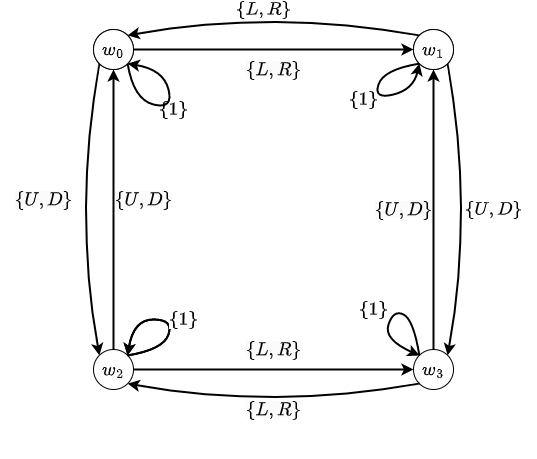
\includegraphics[width=0.5\linewidth]{3ReproducingSBDRL/Old/Images/2x2-cyclical-min-actions-equivalence.png}
    \caption{\sout{Action equivalence classes in $A/\sim$ for the actions show in Figure \ref{fig:2x2-cyclical-min-actions-standard}.}}
    \label{fig:2x2-cyclical-min-act-equivalence}
\end{figure}

\sout{
We define the canonical projection map $\pi_{A}: A \to A/\sim$ that sends actions in $A$ to their equivalence classes under $\sim$ in the set $A/\sim$.
We denote the equivalence class of $a$ by $[a]_{\sim}$.
Sometimes we will drop the $[a]_{\sim}$ in favour of $a \in A/\sim$ for ease.
}

\paragraph{\sout{Composition of actions}}
\sout{
We define the composition of elements in $A/\sim$ as $\circ: (A/\sim) \times (A/\sim) \to (A/\sim)$ such that $[a']_{\sim} \circ [a]_{\sim} = [a' \circ a]_{\sim}$ for $a,a' \in A$.
}

\begin{proposition}
    \sout{
    $[a']_{\sim} \circ [a]_{\sim} = [a' \circ a]_{\sim}$ is well-defined for all $a, a' \in A$.
    }
\end{proposition}
\begin{proof}
    \sout{
    We need to show that the choice of $a,a'$ doesn't matter: if $a_{1} \sim a_{2}$ and $a_{3} \sim a_{4}$ for $a_{1}, a_{2}, a_{3}, a_{4} \in A$, then $[a_{3} \circ a_{1}]_{\sim} = [a_{4} \circ a_{2}]_{\sim}$.
    $a_{1} \sim a_{2}$ means there exists $d_{i}: s(d_{1}) \xrightarrow{a_{i}} t(d_{1})$ for $i=1,2$.
    Since actions are unrestricted in $W$, for any world state and any action there is a transition with a source at that world state that is labelled by that action.
    $a_{3} \sim a_{4}$ means there exists $d_{j}: s(d_{3}) \xrightarrow{a_{j}} t(d_{3})$ for $j=3,4$, and so there exists $d_{j}: t(d_{1}) \xrightarrow{a_{j}} t(d_{3})$ for $j=3,4$.
    $\implies$ there exists $(d_{3} \circ d_{1}): s(d_{1}) \xrightarrow{a_{3} \circ a_{1}} t(d_{3})$ and $(d_{4} \circ d_{2}): s(d_{1}) \xrightarrow{a_{4} \circ a_{2}} t(d_{3})$.
    $\implies$ $s(d_{3} \circ d_{1}) = s(d_{4} \circ d_{2})$ and $t(d_{3} \circ d_{1}) = s(d_{4} \circ d_{2})$.
    $\implies$ $(a_{3} \circ a_{1}) \sim (a_{4} \circ a_{2})$.
    $\implies$ $[a_{3} \circ a_{1})]_{\sim} = [a_{4} \circ a_{2}]_{\sim}$.
    }
\end{proof}

\paragraph{\sout{Effect of equivalent actions on world states}}
\sout{
We define the effect of an element of  $A/\sim$ on world states as $*: (A/\sim) \times W \to W$ such that $[a]_{\sim} * w = a * w$.
Note that this is only defined if there exists $d: w \xrightarrow{a} t(d)$ for $d \in D_{A}$.; if not, then $[a]_{\sim} * w$ is called $\textit{undefined}$.
}

\begin{proposition}
    \sout{
    $[a]_{\sim} * w$ is well-defined for all $a \in A$ and for all $w \in W$.
    }
\end{proposition}
\begin{proof}
    \sout{
    We need to show that $a_{1} * w = a_{2} * w$ if $[a_{1}]_{\sim} = [a_{2}]_{\sim}$ for $a_{1},a_{2} \in A$ and $w \in W$.
    If $[a_{1}]_{\sim} = [a_{2}]_{\sim}$, then $a_{1} \sim a_{2}$.
    Since actions are unrestricted in $W$, for any world state and any action there is a transition with a source at that world state is are labelled by that action.
    $\implies$ there exists $d_{i}: w \xrightarrow{a_{i}} t(d_{1})$ for $i=1,2$.
    $\implies$ $a_{1} * w = d_{1} * w = t(d_{1})$ and $a_{2} * w = d_{2} * w = t(d_{1})$.
    }
\end{proof}

\paragraph{Reversible actions}
An action $a \in A$ is called \textit{reversible} in a given state $w \in W$ if $a \in A_{R w}$ where $A_{Rw} = \{a \in A \mid\textit{ there exists }a' \in A\textit{ such that }a' \circ a * w = w \}$.
An action $a \in A$ is called \textit{reversible} if it is reversible in every $w \in W$.
An action that is not reversible is called \textit{irreversible}.

\paragraph{Properties of the quotient set $A/\sim$}

\begin{proposition}\label{prp:Asim-identity}
    $(A/\sim, \circ)$ has an identity element.
\end{proposition}
\begin{proof}
    To show that $(A/\sim, \circ)$ has an identity element we can show that there is an element $e \in A$ which satisfies (a) $[a]_{\sim} \circ [e]_{\sim} = [a]_{\sim}$ and (b) $[e]_{\sim} \circ [a]_{\sim} = [a]_{\sim}$ for all $a \in A$.
    We will prove that the identity action $1 \in A$ satisfies the above condition.
    Consider any transition $d: s(d) \xrightarrow{a} t(d)$ labelled by any action $a \in A$.
    
    (a) There exists a transition $1_{s(d)}: s(d) \xrightarrow{1} s(d)$ due to action condition \ref{actcon:identity-action}.
    $t(1_{s(d)})=s(d)$ $\implies$ $a \circ 1$ is defined for $d$.
    $s(a \circ 1) = s(1) = s(d) = s(a)$ and $t(a \circ 1) = t(a)$.
    $\implies$ $a \circ 1 \sim a$.
    $\implies$ $[a \circ 1]_{\sim} = [a]_{\sim}$.
    $\implies$ $[a]_{\sim} \circ [1]_{\sim} = [a]_{\sim}$.
    
    (b) There exists a transition $1_{t(d)}: t(d) \xrightarrow{1} t(d)$ due to action condition \ref{actcon:identity-action}.
    $t(1_{t(d)})=t(d)$ $\implies$ $1 \circ a$ is defined for $d$.
    $s(1 \circ a)=s(a)$ and $t(1 \circ a) = t(1) = t(a)$.
    $\implies$ $1 \circ a \sim a$.
    $\implies$ $[1 \circ a]_{\sim} = [a]_{\sim}$.
    $\implies$ $[1]_{\sim} \circ [a]_{\sim} = [a]_{\sim}$.
    Therefore $1 \in A$ satisfies the conditions for $[1]_{\sim}$ being an identity element in $(A/\sim, \circ)$.
\end{proof}

\begin{proposition}\label{prp:Asim-associative}
    $\circ$ is associative with respect to $(A/\sim, \circ)$.
\end{proposition}
\begin{proof}
    For $\circ$ to be associative we need $[a_{1}]_{\sim} \circ ([a_{2}]_{\sim} \circ [a_{3}]_{\sim}) = ([a_{1}]_{\sim} \circ [a_{2}]_{\sim}) \circ [a_{3}]_{\sim}$ for any $a_{1},a_{2},a_{3} \in A$.
    We have $a_{1} \circ (a_{2} \circ a_{3}) = (a_{1} \circ a_{2}) \circ a_{3}$ from the associativity of $\circ$ with respect to $(A, \circ)$, and $[a']_{\sim} \circ [a]_{\sim} = [a' \circ a]_{\sim}$ for any $a,a' \in A$ by definition of $\circ$ on $A/\sim$.
    $\implies$ $[a_{1}]_{\sim} \circ ([a_{2}]_{\sim} \circ [a_{3}]_{\sim}) = [a_{1} \circ (a_{2} \circ a_{3})]_{\sim} = [(a_{1} \circ a_{2}) \circ a_{3}]_{\sim} = [(a_{1} \circ a_{2})]_{\sim} \circ [a_{3}]_{\sim} = ([a_{1}]_{\sim} \circ [a_{2}]_{\sim}) \circ [a_{3}]_{\sim}$.
\end{proof}

In summary, we have $(A, \circ, *)$, which is a set $A$ along with two operators $\circ: A \times A \to A$ and $*: A \times W \to W$, and we have $(A/\sim, \circ, *)$, which is a set $A/\sim$ along with two operators $\circ: (A/\sim) \times (A/\sim) \to (A/\sim)$ and $*: (A/\sim) \times W \to W$.
We have shown that $\circ$ is associative with respect to $(A/\sim, \circ)$, and that $(A/\sim, \circ)$ has an identity element by action condition \ref{actcon:identity-action}.


%%%%%%%%%%%%%%%%%%%%%%%%%%%%%%%%%%%%%%%%%%%%%%%%%%%%%%%%%%%%%%%%%%%%%%%%%%%%%%%%%%%%%%%%
\subsection{Conditions for SBDRL to apply}\label{sec:World conditions}

To simplify the problem, we only consider worlds where the transformations of the world are only due to the actions of an agent for the remainder of this paper unless otherwise stated; this means we do not have to take into consideration how the agent would deal with transformations of the world, not due to its actions.
Therefore, we will only consider worlds with $D = D_{A}$.

To be a group, $A/\sim$ must satisfy the properties of (1) identity, (2) associativity, (3) closure, and (4) inverse.
(1) The identity property and (2) the associativity property are satisfied by Proposition \ref{prp:Asim-identity} and Proposition \ref{prp:Asim-associative} respectively.
(3) For the closure property to be satisfied, the following condition is sufficient:
\begin{world_condition}[Unrestricted actions]\label{wldcon:unrestricted-actions}
    For any action $a \in A$ and for any world state $w \in W$, there exists a transition $d \in D_{A}$ with $d: w \xrightarrow{a} t(d)$.
    In other words, $a * w$ is defined for all $a \in A$ and all $w \in W$.

    \whendraft{
    \textit{Mathematically:} For any $w_{i} \in W$, there exists $a \in A$ and $w_{j} \in W$ such that $a * w_{i} = w_{j}$.
    }
\end{world_condition}

The inverse property of a group is more strict than our current definition of the reversibility of an action.
For the structure $A/\sim$ to have the inverse property, each element (action) in $A/\sim$ must not only be reversible from each starting state, but additionally, the inverse of a given element in $A/\sim$ must be the same for each starting state; for example, if $a'$ is the inverse of $a$ from a state $w \in W$ ($a' \circ a * w = w$), then $a'$ must be the inverse of $a$ from all states in $W$.

\begin{world_condition}[Inverse actions]\label{wldcon:inverse-actions}
    For each $a \in A/\sim$, there exists an $a' \in A/\sim$ such that $a' \circ a * w = w$ and $a \circ a' * w = w$ for all $w \in W$.
\end{world_condition}


\begin{proposition}\label{prp:Asim-group}
    If the world satisfies world conditions \ref{wldcon:unrestricted-actions} and \ref{wldcon:inverse-actions} then $(A/\sim, \circ)$ is a group.
\end{proposition}
\begin{proof}
    \whendraft{
    [\textbf{Update this proof}]
    }
    Totality is given by world condition \ref{wldcon:unrestricted-actions}.
    Associativity is given by proposition \ref{prp:Asim-associative}.
    Identity element given by proposition \ref{prp:Asim-identity}.
    Inverse element is given by world condition \ref{wldcon:inverse-actions}.
\end{proof}

\begin{proposition}\label{prp:world-conditions-sufficient}
    If the world obeys world conditions \ref{wldcon:unrestricted-actions} and \ref{wldcon:inverse-actions}, then $*: (A/\sim) \times W \to W$ is a left group action.
\end{proposition}
\begin{proof}
    \whendraft{
    [\textbf{Update this proof}]
    }
    We have already established that $(A/\sim, \circ)$ is a group (proposition \ref{prp:Asim-group}).
    Therefore, to show that $*$ is a left group action we only have to prove the group action conditions of (a) identity and (b) compatibility.
    Consider an arbitrary world state $w \in W$.
    
    (a) $[1]_{\sim} * w = 1 * w = 1_{w} * w = w$.
    
    (b) We need to show that $a' * (a * w) = (a' \circ a) * w$.
    Because actions are unrestricted in $W$, for any $w \in W$, there exists the transitions $d_{1}: w \xrightarrow{a} t(d_{1})$ and $d_{2}: t(d_{1}) \xrightarrow{a} t(d_{2})$.
    $\implies$ there exists the transition $(d_{2} \circ d_{1}): w \xrightarrow{a' \circ a} t(d_{2})$.
    Therefore, $(a' \circ a) * w = t(d_{2})$.
    Using the transitions $d_{1}$ and $ d_{2}$ for the LHS of the condition, $a' * ( a * w) = a' * t(d_{1}) = t(d_{2})$.
\end{proof}

From Proposition \ref{prp:world-conditions-sufficient}, if a world satisfies world conditions \ref{wldcon:unrestricted-actions} and \ref{wldcon:inverse-actions}, then the transformations of that world can be fully described using SBDRL (\textit{i.e.}, $*: (A/\sim) \times W \to W$ is a group action).

\begin{proposition}\label{prp:unrestricted-actions-necessary}
    If $*: (A/\sim) \times W \to W$ is a group action, then world condition \ref{wldcon:unrestricted-actions} is satisfied.
\end{proposition}
\begin{proof}
    Since a group action is a full operation by definition,  world condition \ref{wldcon:inverse-actions} is satisfied.
\end{proof}

\begin{proposition}\label{prp:inverse-actions-sufficient}
    If $*: (A/\sim) \times W \to W$ is a group action, then world condition \ref{wldcon:inverse-actions} is satisfied.
\end{proposition}
\begin{proof}
    If $*$ is a group action, 
    then $A/\sim$ is a group.
    If $A/\sim$ is a group, then for each $a \in A/\sim$ there is an inverse element $a^{-1}$ such that (1) $a^{-1} \circ a = 1$ and (2) $a \circ a^{-1} = 1$.

    For an arbitrary state $w \in W$, $a^{-1} \circ (a * w) = a^{-1} \circ (a * w)$, therefore $a^{-1} \circ (a * w) = (a^{-1} \circ a) * w$ from the group action compatibility condition, therefore  $a^{-1} \circ (a * w) = 1 * w$ from (1), therefore (3) $a^{-1} \circ (a * w) = w$ from the group action identity condition.

    Similarly, for an arbitrary state $w \in W$, $a \circ (a^{-1} * w) = a \circ (a^{-1} * w)$, therefore $a \circ (a^{-1} * w) = (a \circ a^{-1}) * w$ from the group action compatibility condition, therefore $a \circ (a^{-1} * w) = 1 * w$ from (2), therefore (4) $a \circ (a^{-1} * w) = w$ from the group action identity condition.

    (3) and (4) together are world condition \ref{wldcon:inverse-actions}.
\end{proof}


\begin{proposition}\label{prp:WC-unrestricted-actions-necessary}
    If a world does not satisfy world condition \ref{wldcon:unrestricted-actions}, then $*$ is not a group action.
\end{proposition}
\begin{proof}
    If a world does not satisfy world condition \ref{wldcon:unrestricted-actions}, then there exists some world state $w \in W$ and some action $a \in A$ such that $a * w$ is undefined.
    Therefore, for $[a] \in A/\sim$, $[a] * w$ is undefined, and so $*: (A/\sim) \times W \to W$ is a partial operation and so not a group action.
\end{proof}


\begin{proposition}\label{prp:WC-inverse-actions-necessary}
    If a world does not satisfy world condition \ref{wldcon:inverse-actions}, then $A/\sim$ is not a group and so $*$ is not a group action.
\end{proposition}
\begin{proof}
    If a world does not satisfy world condition \ref{wldcon:inverse-actions}, then there exists an $a \in A/\sim$ such that there is no $a' \in A/\sim$ for which $a' \circ a * w = w$ or $a \circ a' * w = w$ for all $w \in W$.
    \textbf{Proof by contradiction.}
    Assume $a$ has an inverse $a'' \in A/\sim$.
    Therefore, $a'' \circ a \sim 1$ and $a \circ a'' \sim 1$.
    Since $1 * w = w$ for all $w \in W$, $a'' \circ a * w = w$ and $a \circ a'' * w = w$ for all $w \in W$, which is a contradiction.
\end{proof}


Proposition \ref{prp:world-conditions-sufficient} shows that world conditions \ref{wldcon:unrestricted-actions} and \ref{wldcon:inverse-actions} are sufficient conditions for $*$ to be a group action, while propositions \ref{prp:WC-unrestricted-actions-necessary} and \ref{prp:WC-inverse-actions-necessary} show that world conditions \ref{wldcon:unrestricted-actions} and \ref{wldcon:inverse-actions} are necessary conditions for $*$ to be a group action.
Since world conditions \ref{wldcon:unrestricted-actions} and \ref{wldcon:inverse-actions} are sufficient and necessary conditions for $*$ to be a group action and therefore $A/\sim$ to be a group, these conditions give a characterisation of the worlds with transformations (due to the actions of an agent) that can be fully described using SBDRL; in other words, if the transformations of a world can be fully described using SBDRL then that world satisfies world conditions \ref{wldcon:unrestricted-actions} and \ref{wldcon:inverse-actions}, and if a world satisfies world conditions \ref{wldcon:unrestricted-actions} and \ref{wldcon:inverse-actions} then the transformations of that world can be fully described using SBDRL.

%%%%%%%%%%%%%%%%%%%%%%%%%%%%%%%%%%%%%%%%%%%%%%%
\subsection{Action-homogeneous worlds\whendraft{ and generalisation potential}}

\whendraft{
\begin{proposition}
    If $A/\sim$ is a group, then $a' \circ a * w = w$ ($w \in W$, $a, a' \in A/\sim$) does not mean that $a' \circ a * w' = w'$ for all $w' \in W$.
\end{proposition}
\begin{proof}
    Proof by counter example.
    Consider the world given in Figure ?
    [insert figure here]
    The algebra of the actions of an agent with minimum actions $\{1, a, b\}$ is given by the following action Cayley table:
    [insert action Cayley table]
\end{proof}
}

\begin{world_condition}[Action homogeneity]\label{wldcon:action-homogeneity}
    For every pair $(w_{1}, w_{2}) \in W^{2}$, there exists a bijective map $\sigma_{(w_{1},w_{2})}: W \to W$ such that $\sigma_{(w_{1},w_{2})}(w_{1})=w_{2}$ and such that:
    
    \begin{enumerate}
        \item for every $d \in D_{A}$ with $d: s(d) \xrightarrow{a} t(d)$, there exists a $d' \in D_{A}$ with $d': \sigma_{(w_{1}, w_{2})}(s(d)) \xrightarrow{a} \sigma_{(w_{1}, w_{2})}(t(d))$;
        
        % Is this part needed --> implied by first condition due to $\sigma$ being a bijection ?
        \item for every $d \in D_{A}$ with $d: s(d) \xrightarrow{a} t(d)$, there exists a $d' \in D_{A}$ with $d': \sigma^{-1}_{(w_{1}, w_{2})}(s(d)) \xrightarrow{a} \sigma^{-1}_{(w_{1}, w_{2})}(t(d))$.
    \end{enumerate}
\end{world_condition}

World condition \ref{wldcon:action-homogeneity} means that action sequences have the same result for any initial world state.
Essentially, this means that the world looks the same from any world state with respect to the relationships of actions.
We call worlds with world condition \ref{wldcon:action-homogeneity} \textit{action-homogeneous worlds}.

\begin{definition}[Weak equivalence $\sim_{w}$]\label{def:weak action equivalence}
    For $a,a' \in A$ and $w \in W$, $a \sim_{w} a$ if $a * w = a' * w$ or $a$ and $a'$ are both restricted actions with respect to $w$.
\end{definition}

\begin{remark}
    In definition \ref{def:weak action equivalence}, for the case where $a, a'$ are both restricted actions, then we say $a * w = a' * w$.
    The meaning of $a * w$ where $a$ is restricted on $w$ will be defined later.
\end{remark}

\begin{proposition}
    $\sim_{w}$ is an equivalence relation.
\end{proposition}
\begin{proof}
    To show that $\sim_{w}$ is an equivalence relation, we need to show that the relation is (a) reflexive, (b) transitive, and (c) symmetric.
    (a) For a binary relation $R$ over a set $X$ to be reflexive: $x R x$ for every $x \in X$.
    For $w \in W$, if $a * w$ is defined then $a * w = a * w$ from the properties of $=$ for any $a \in A$.
    Therefore, $a \sim_{w} a$.
    (b) For a binary relation $R$ over a set $X$ to be transitive: if $a R b$ and $b R c$ then $a R c$ for all $a,b,c \in X$.
    If $a \sim_{w} a'$ and $a' \sim_{w} a''$, then $a * w = a' * w$, $a' * w = a'' * w$ for all $w \in W$.
    Combining these two equations gives $a * w = a'' * w$.
    (c) For a binary relation $R$ over a set $X$ to be reflexive: if $a R b$, then $b R a$ for all $a,b \in X$.
    If $a \sim_{w} a'$, then $a * w = a' * w$. Therefore $a' * w = a * w$, and so $a' \sim_{W} a$.
\end{proof}


For action-homogeneous worlds, the following properties hold:
\begin{enumerate}
    \item If a world is action-homogeneous, then $a \sim_{w} a'$ means $a \sim a'$ - this makes it much easier to learn the algebra of action-homogeneous worlds;
    
    \item The number of elements in $A/\sim$ is always equal to the number of states in the world since for any state $w \in W$, there is exactly one action $a \in A/\sim$ for which $a * w = w'$ where $w'$ is any state in $W$; therefore the number of elements in the action algebra is equal to the number of states in $W$;
    
    \item If $a * w_{i} = w_{j}$, then there exists a world state $w_{k} \in W$ such that $a * w_{k} = w_{i}$.
    In other words, if $a$ is defined from one world state it is defined from all world states;

    \item If $a' * (a * w) = a * (a' * w) = w$ for any $w \in W$, then $a' * (a * w) = a * (a' * w) = w$ for all $w \in W$.
    In other words, reversible actions imply inverse actions.
\end{enumerate}

\whendraft{
\textbf{[Insert info about generalisation.]}
\begin{itemize}
    \item If we know that, from a particular initial state, a particular sequence of actions has a particular outcome and we know that a different sequence of actions from the same initial state has the same outcome then we know that those two action sequences will have the same outcome in from every initial state (and therefore will be equivalent?!).
    \begin{itemize}
        \item Illustrate this using the counter-example - see PhD Notebook 1 notes.
    \end{itemize}
\end{itemize}
}

%%%%%%%%%%%%%%%%%%%%%%%%%%%%%%%
\subsection{Summary}
In summary, we have presented a mathematical formalism for describing transitions and actions of an agent between world states.
We have then given an example world and shown that, after applying an equivalence relation, the algebra of the actions of the agent in this example world forms a group.
We have also characterised the worlds with transformations that can be fully described by SBDRL by giving world conditions that are sufficient and necessary for the algebra of the transformations of that world to be a group.
Finally, we have introduced the concept of action homogeneity, which has allowed us to identify a collection of worlds for which it should be easier to learn action algebras.

}
